%!TEX root = draft.tex
\section{Computing ADT Complements}
\label{sec:patterns}

TODO MOTIVATE THIS SECTION; ALSO, RETHINK THE TITLE OF THIS SECTION

In addition to the relations $\to_\mathrm{o}$, $\to_\mathrm{p}$, and
$\to_\mathrm{c}$ of Section~\ref{sec:histories} under which all ADTs are
closed, the ADTs we consider in this work are also closed under additional
relations which remove read-only operations, unmatched operations, entire
matches, and duplicate operations. The relations $\to_\mathrm{r}$,
$\to_\mathrm{u}$, $\to_\mathrm{m}$ and $\to_\mathrm{d}$ relate two histories
$h_1$ and $h_2$ when $h_2$ is obtained from $h_1$ by
\begin{itemize}

  \item removing a read-only operation (r),

  \item removing an unmatched operation (u),

  \item removing a match (m), or

  \item removing a duplicate operation (d).

\end{itemize}
We say an ADT closed under $\to_\mathrm{r}$, $\to_\mathrm{u}$, $\to_\mathrm{m}$
and $\to_\mathrm{d}$ is \emph{normal}. In Section~\ref{sec:nature} we
demonstrate that naturally-occurring ADTs are normal. Defining the relation
$\succeq$ as the reflexive and transitive closure of the above relations,
\begin{align*}
  \mathord{\succeq} = (
    \to_\mathrm{o} \cup \to_\mathrm{p} \cup \to_\mathrm{c} \cup 
    \to_\mathrm{r} \cup \to_\mathrm{u} \cup \to_\mathrm{m} \cup \to_\mathrm{d}
  )^\ast
\end{align*}
closure under $\succeq$ follows immediately.

\begin{lemma}

  Normal ADTs are closed under $\succeq$.

\end{lemma}

TODO MOTIVATE WQO

A \emph{well-quasi-ordering (wqo)} $R$ on a set $X$ is a reflexive, transitive
binary relation on $X$ for which in every infinite sequence $x_0 x_1 \ldots$ of
elements from $X$, there exists indices $i < j$ such that $R(x_i,x_j)$.

\begin{example}

  Consider the infinite history sequence $h_1 h_2 \ldots$ where each $h_i$
  contains $2i$ operations $o_1, o_1', \ldots, o_i, o_i'$ where each $o_j$ is a
  completed {\tt push} operation matching itself, and each $o_j'$ is a pending
  {\tt pop} operation with undefined matching. Because each successive $h_i$
  has both more matches and more pending operations, no two histories of the
  sequence are related by $\preceq$. Thus $\preceq$ is not a wqo.

\end{example}

The previous example demonstrates that $\preceq$ is not a wqo by allowing each
history $h_i$ of the infinite sequence to contain more and more pending
operations in order to ensure that $h_j \not\preceq h_i$ for every $j < i$.
Curbing this ability by limiting the maximum amount of pending operations per
history makes $\preceq$ a wqo. Although limiting to $k$ pending operations
essentially limits us to width-$k$ histories, of executions with at most $k$
operations parallel at any moment, e.g.,~of programs with at most $k$ threads,
this restriction comes at no loss of completeness when considering only the
histories of bounded-width ADT kernels, which is the subject of the remainder
of this section.

We first prove that the embedding order, defined hereafter, is a wqo on width-bounded
labeled interval orders.

Let $\Sigma$ be a finite alphabet. A labeled interval order is a triple $(A,\leq,\ell)$, where $(A,\leq)$ is an interval 
order, and $\ell:A\rightarrow \Sigma$ is a labeling function. The embedding order $\subseteq$ between labeled interval orders is defined as
usual by:
\begin{itemize}
	\item $(A_1,\leq_1,\ell_1)\subseteq (A_2,\leq_2,\ell_2)$ iff there exists an injective function $h:A_1\rightarrow A_2$ that 
	preserves the labeling, i.e., $\ell_1(x)=\ell_2(h(x))$, for every $x\in A_1$, and the order constraints, i.e.,
	for every $x,y\in A_1$, if $x \leq_1 y$, then $h(x)\leq_2 h(y)$.
\end{itemize}

The width of an interval order $(A,\leq,\ell)$ is the maximum number of elements which are mutually unordered.

\begin{lemma}
$\subseteq$ is a wqo on width-bounded interval orders.
\end{lemma}
\begin{proof}
By definition, for every interval order $(A,\leq,\ell)$, there exists a mapping $I$ from elements of $A$ to intervals over $\mathbb{N}$ such that for every $x,y\in A$, if $x\leq y$, then the interval $I(x)$ ends before the interval $I(y)$ (i.e., the upper bound of $I(x)$ is strictly smaller than the lower bound of $I(y)$). %In general, there are more than one mappings $I_A$ that satisfy these constraints. In the following, we assume that the mapping $I_A$ is arbitrary but fixed.
Therefore, in the following, we assume that an interval order is a multiset $\Gamma$ of triples of the form $[i,j,a]$ where $[i,j]$ is an interval on the integer line and $a$ is a symbol in $\Sigma$.

We prove that another order on interval orders, denoted by $\subseteqq$, which is stronger than the embedding order $\subseteq$, is a wqo. The order $\subseteqq$ is defined by: $\Gamma_1\subseteqq \Gamma_2$ iff there exists an injective function $h:\Gamma_1\rightarrow \Gamma_2$ such that 
\begin{enumerate}
	\item $h$ preserves the labeling, i.e., for any triple $[i,j,a]$, $h([i,j,a])=[i',j',a]$, for some $i'$, $j'$, 
	\item $h$ preserves the ordering constraints, i.e., for every two triples $[i,j,a]$ and $[k,l,b]$ such that $j< k$, $h([i,j,a])=[i',j',a]$, $h([k,l,b])=[k',l',b]$, and $j'< k'$.
	\item for every two incomparable elements $x$ and $y$ of $\Gamma_1$, if the interval of $x$ starts before the interval of $y$, then the interval of $h(x)$ also starts before the interval of $h(y)$. Formally, for every two triples $[i,j,a]$ and $[k,l,b]$ such that $i\leq k$ (i.e., the first interval starts before the second interval), $h([i,j,a])=[i',j',a]$, $h([k,l,b])=[k',l',b]$, and $i'\leq k'$.
\end{enumerate}
		
Assume $\Gamma_1$, $\Gamma_2$,$\ldots$ is a \emph{bad} sequence, i.e., an infinite sequence of interval orders s.t. there exists no $i < j$ with $\Gamma_i\subseteqq \Gamma_j$. Also, assume that $\Gamma_1$ is the minimal size interval order that can start a bad sequence, $\Gamma_2$ is the minimal interval order that can continue a bad sequence starting with $\Gamma_1$, and so on.

For each $\Gamma_k$, let $Min(\Gamma_k)$ be a triple $[i,j,a]$ such that 
\begin{itemize}
	\item $i$ is the minimal lower bound of an interval in $\Gamma_k$, and 
	\item $j$ is the minimal upper bound of an interval in $\Gamma_k$ with lower bound $i$.
\end{itemize}
%In general, this triple is not unique but it’s not important which one we choose.

Also, let $Init(\Gamma_k) = (Min(\Gamma_k), P_k)$, where $P_k$ is the multiset of symbols labeling elements of $\Gamma_k$ that are incomparable to $Min(\Gamma_k)$. Note that $P_k$ is bounded since we assume width-bounded interval orders.

The infinite sequence $\Gamma_1$, $\Gamma_2$,$\ldots$ contains an infinite sequence $\Gamma_{k_1}$, $\Gamma_{k_2}$,$\ldots$ which, ignoring the integer interval, have the same value for $Init$.

For each $\Gamma_k$, let $\Lambda_k$ be the interval order obtained from $\Gamma_k$ by removing the triple $Min(\Gamma_k)$.

By the minimality assumptions, the infinite sequence $\Gamma_1$, $\Gamma_2$,$\ldots$,$\Gamma_{k_1-1}$, $\Lambda_{k_1}$, $\Lambda_{k_2}$,$\ldots$ is not bad. 
Therefore, there exists $m<n$ such that $\Lambda_{k_m}\subseteqq \Lambda_{k_n}$. 

It remains to prove that:
\begin{itemize}
	\item if $Init(\Gamma_{k_m})=Init(\Gamma_{k_n})$ and $\Lambda_{k_m}\subseteqq \Lambda_{k_n}$, then $\Gamma_{k_m}\subseteqq \Gamma_{k_n}$.
\end{itemize}

Let $h$ be the injective function witnessing $\Lambda_{k_m}\subseteqq \Lambda_{k_n}$. We prove that the extension $h'$ of $h$ between $\Gamma_{k_m}$ and $\Gamma_{k_n}$, defined by $h'(Min(\Gamma_{k_m}))=Min(\Gamma_{k_n}$ and $h'(t)=h(t)$, for all $t\in \Lambda_{k_m}$ witnesses $\Gamma_{k_m}\subseteqq \Gamma_{k_n}$. Clearly, $h'$ preserves the labeling. 

To prove that $h'$ preserves the ordering constraints, let $Min(\Gamma_{k_m})=[i,j,a]$ and $[k,l,b]\in \Gamma_{k_m}$ such that $j< k$. Also, let $Min(\Gamma_{k_n})=[i',j',a]$ and $h'([k,l,b])=h([k,l,b])=[k',l',b]$. Assume by contradiction that $k'\leq j'$. Since $h$ is injective, there exists an element $[x,y,c]\in \Gamma_{k_m}$ incomparable to $Min(\Gamma_{k_m})$ which is mapped to an element $[x',y',c]$ greater than $Min(\Gamma_{k_n})$ (by definition, $\Gamma_{k_m}$ and $\Gamma_{k_n}$ have the same number of elements incomparable to $Min(\Gamma_{k_m})$ and respectively, $Min(\Gamma_{k_n})$). 
Since $[x,y,c]$ is incomparable to $[i,j,a]$, we obtain that $x\leq j< k$. Also, by the current assumptions, $k'<j'<x'$. Therefore, there exist two elements $[x,y,c]$ and $[k,l,b]$ such that the interval $[x,y]$ starts before $[k,l]$ which are mapped by $h$ to the elements $[x',y',c]$ and $[k',l',b]$ such that the interval $[x',y']$ starts after $[k',l']$. This contradicts the fact that $h$ witnesses $\Lambda_{k_m}\subseteqq \Lambda_{k_n}$.

The properties of $Min(\Gamma_{k_m})$ and $Min(\Gamma_{k_n})$ imply that $h'$ also satisfies the third property in the definition of $\subseteqq$.

Finally, since $\subseteqq$ is stronger than $\subseteq$, we get that $\subseteq$ is a wqo on width-bounded labeled interval orders.
\end{proof} 

\begin{lemma}

  $\preceq$ is a wqo on width-bounded histories.

\end{lemma}

\begin{proof}

%We prove that $\preceq$ is well-founded, i.e., there is no infinite strictly decreasing sequence $h_1 \succ h_2\succ \ldots$\footnote{We define $\succ$ as usual by $h\succ h'$ iff $h\succeq h'$ and $h\neq h'$.},
%and that $\preceq$ has no infinite antichain, i.e., there is no infinite set $\{h_1,h_2,\ldots\}$ of mutually incomparable elements 
%$h_i\not\preceq h_j$ and $h_j\not\preceq h_i$ when $i\neq j$.
%
%Concerning well-foundedness, note that a given history $h_1$ can be weaken only finitely many times by removing matches, duplicates in a match, or happens-before ordering constraints, or by turning completed operations into pending operations. Since we restrict ourselves to width-bounded histories, $h_1$ can also be weaken only finitely many times by adding pending operations (adding a pending operation increases the width of a history by 1).
%
%TODO PROBLEM WITH PENDING OPS

%To prove that $\preceq$ has no infinite antichain, 
%we use the following definitions.
Let $h_1 h_2\ldots $ be an infinite sequence of histories. We prove that there exists $i<j$ such that $h_i\preceq h_j$.

The \emph{signature} of an operation $o$ in a history $h$ is the pair $\sigma(o)=(c(o),f(o))$.
Then, the \emph{signature} of a match $\mu=\set{ o' \in O : m(o') = o}$ is the pair 
\[
\sigma(\mu)=(\sigma(o),\set{\sigma(o') : m(o')=o, o'\neq o})
\]
containing the signature of the match target and the set of the signatures of the other operations.
The \emph{signature} of a history $h$ is the tuple 
\begin{align*}
\sigma(h)&=&(\set{\sigma(\mu): \mu\mbox{ a match}}, \set{\sigma(o): o\mbox{ read-only}}, \\
&& \set{\sigma(o): o\mbox{ completed and unmatched}}, \\
&& \mset{\sigma(o): o\mbox{ pending and unmatched}}).
\end{align*}

The history signature contains sets of signatures 
(for matches, read-only and respectively, completed and unmatched operations) 
and the multiset of signatures of the pending and unmatched operations.

%Assume by contradiction that $\preceq$ has an infinite antichain.
Since the set of history signatures is bounded (because the set of methods is bounded)
and the set of pending operations is also bounded (since we consider only bounded width histories),
the sequence $h_1 h_2\ldots $ contains an infinite sequence of histories $h_1' h_2' \ldots$ that have 
the same signature. 

%
%Also, 

The \emph{vector} of a history $h$ is the tuple
\begin{align*}
\nu(h)&=&(\mset{\sigma(\mu): \mu\mbox{ a match of $h$}}, \mset{\sigma(o): o\mbox{ read-only}}, \\
&& \mset{\sigma(o): o\mbox{ completed and unmatched}}).
\end{align*}

Let $\leq$ be an order relation on multisets $\alpha:\Sigma\rightarrow\mathbb{N}$ of (match or operation) signatures from a finite set $\Sigma$ 
defined by $\alpha\leq\alpha'$ iff $\alpha(\sigma)\leq\alpha'(\sigma)$, for every $\sigma\in\Sigma$.
Clearly, $\leq$ is a wqo and so is the component-wise extension of $\leq$ to history vectors.
Therefore, by known results, the sequence of histories $h_1' h_2' \ldots$ contains 
an infinite sequence $h_1'',h_2'',\ldots$ such that $\nu(h_1'')\leq \nu(h_2'')\leq \ldots$.

The \emph{vector} of a match $\mu$ is the pair
\[
\nu(\mu)=(\sigma(o),\mset{\sigma(o') : m(o')=o, o'\neq o})
\]
containing the signature of the match target and the multiset of the signatures of the other operations.

For every history $h$ and match signature $\sigma$, the \emph{$\sigma$-vector} of a history $h$ is the multiset
\[
\nu_\sigma(h)=\mset{\nu(\mu): \sigma(\mu)=\sigma}
\]
of match vectors of signature $\sigma$.

Let $\leq_v$ be an order relation on $\sigma$-vectors defined by $\nu_\sigma(h)\leq_v \nu_\sigma(h')$ iff
\begin{itemize}
	\item for every match vector $\nu$ in $\nu_\sigma(h)$ there exists a match vector $\nu'$ in $\nu_\sigma(h')$
	such that $\nu\leq \nu'$ (here, $\leq$ is the order on multisets defined above).
\end{itemize}
By known results, $\leq_v$ is a wqo.

Let $\sigma_1$, $\sigma_2$,$\ldots$, $\sigma_n$ be the match signatures defined over a set of methods $\mathbb{M}$.
Since $\leq_v$ is a wqo, the sequence of histories $h_1'',h_2'',\ldots$ contains an 
infinite sequence $h_{1}^1,h_{2}^1,\ldots$ such that 
$\nu_{\sigma_1}(h_{1}^1)\leq_v \nu_{\sigma_1}(h_{2}^1)\leq_v \ldots$.
Then, the sequence $h_{1}^1,h_{2}^1,\ldots$ contains 
an infinite sequence $h_{1}^2,h_{2}^2,\ldots$ such that 
$\nu_{\sigma_2}(h_{1}^2)\leq_v \nu_{\sigma_2}(h_{2}^2)\leq_v \ldots$.
Applying a similar reasoning for the rest of the match signatures, 
we obtain that $h_1'',h_2'',\ldots$ contains an 
infinite sequence $h_{1}^n,h_{2}^n,\ldots$
such that 
$\nu_{\sigma}(h_{1}^n)\leq_v \nu_{\sigma}(h_{2}^n)\leq_v \ldots$, for every signature $\sigma$.
Recall that we also have that
$\nu(h_1^n)\leq\nu(h_2^n)\leq\ldots$ since $h_{1}^n,h_{2}^n,\ldots$ is a sub-sequence of $h_1'',h_2'',\ldots$.

Viewing histories as labeled interval orders, where the label of an element $o$ is the triple $(c(o),f(o),r(o))$,
we get that the embedding order $\subseteq$ is a wqo on histories. Therefore, the infinite sequence
$h_{1}^n,h_{2}^n,\ldots$  contains two elements $h_{i}^n$ and $h_j^n$ with $i<j$ such that $h_{i}^n\subseteq h_j^n$.
This implies that $h_i^n\preceq h_j^n$, which ends our proof.
\end{proof}

For the remainder of this section, we fix an ADT $A$, and let $B$ be the
complement of $\ker A$. When $\ker A$ has bounded width, so does $B$, and thus
$\preceq$ is a wqo on $B$. Furthermore, when $A$ normal, it is closed under
$\succeq$, and thus $B$ is closed under $\preceq$. Closure under a wqo implies
representation by a finite set. Formally, we say a set $X$ is \emph{finitely
representable} if there exists a finite set $Y$ and a relation $R \subseteq Y
\times X$ such that $X = \set{ x : \exists y\in Y.\ R(y,x) }$. In our case, we
obtain a finite set from which exactly the elements of $B$ are related by
$\preceq$.

\begin{lemma}

  $B$ is finitely representable if $A$ is normal.

\end{lemma}

Computing $B$ thus amounts to computing its finite representation. In general,
this is achieved by enumerating the elements of $B$ while maintaining the
$\preceq$-minimal elements, and recognizing a condition under which all
elements of $B$ are related to the current set of
minimals~\cite{conf/lics/AbdullaCJT96, journals/tcs/FinkelS01}. In our case, we
recognize a condition on the weight-increasing enumeration of $B$ which
guarantees coverage by the current set of minimals. Formally, for all $i \in
\mathbb{N}$, we define
\begin{align*}
  B_i &= \set{ h \in B : \weight(h) \le i } \\
  B_i' &= \set{ h' \in B :
    \exists h \in B_i.\ h \preceq h' \text{ and } \weight(h') \le i+1
  }
\end{align*}
as, respectively, the histories of $B$ with at most $i$ matches and duplicates,
and those derived from $B_i$ with at most $i\!+\!1$ matches and duplicates. We
say that $A$ is \emph{predictable} if $B_i = B$ whenever $B_i' = B_{i+1}$. In
Section~\ref{sec:nature} we demonstrate that naturally-occurring ADTs are
predictable. Since the number of weight-$i$ histories is finite\footnote{As
noted in Section~\ref{sec:histories}, we consider equality between histories up
to renaming of operation identifiers.} for each $i \in \mathbb{N}$, each $B_i$
is computable.

\begin{lemma}

  $B_i$ is computable, for all $i \in \mathbb{N}$, if $A$ is normal.

\end{lemma}

Predictability ensures that once $B_{i+1}$ does not alter the set of computed
$\preceq$-minimals, with respect to those of $B_i$, then the minimals computed
for $B_i$ are exactly those of $B$.

\begin{lemma}

  $B$ is computable if $A$ is normal and predictable.

\end{lemma}

Note that for non-predictable ADTs, computing $B_i$, for any $i \in
\mathbb{N}$, under-approximates $B$. In practice, computing $B_i$ can be used
to identify all violations which surface in histories with $i$ matches,
overlooking violations which only surface with more than $i$ matches. The
resulting symbolic ADT representation would still be sound in only identifying
\emph{actual} violations, yet incomplete in identifying \emph{all} violations.

\begin{example}

  TODO EXAMPLE OF COMPLETE PATTERNS

  \begin{figure}[t]
    \centering
    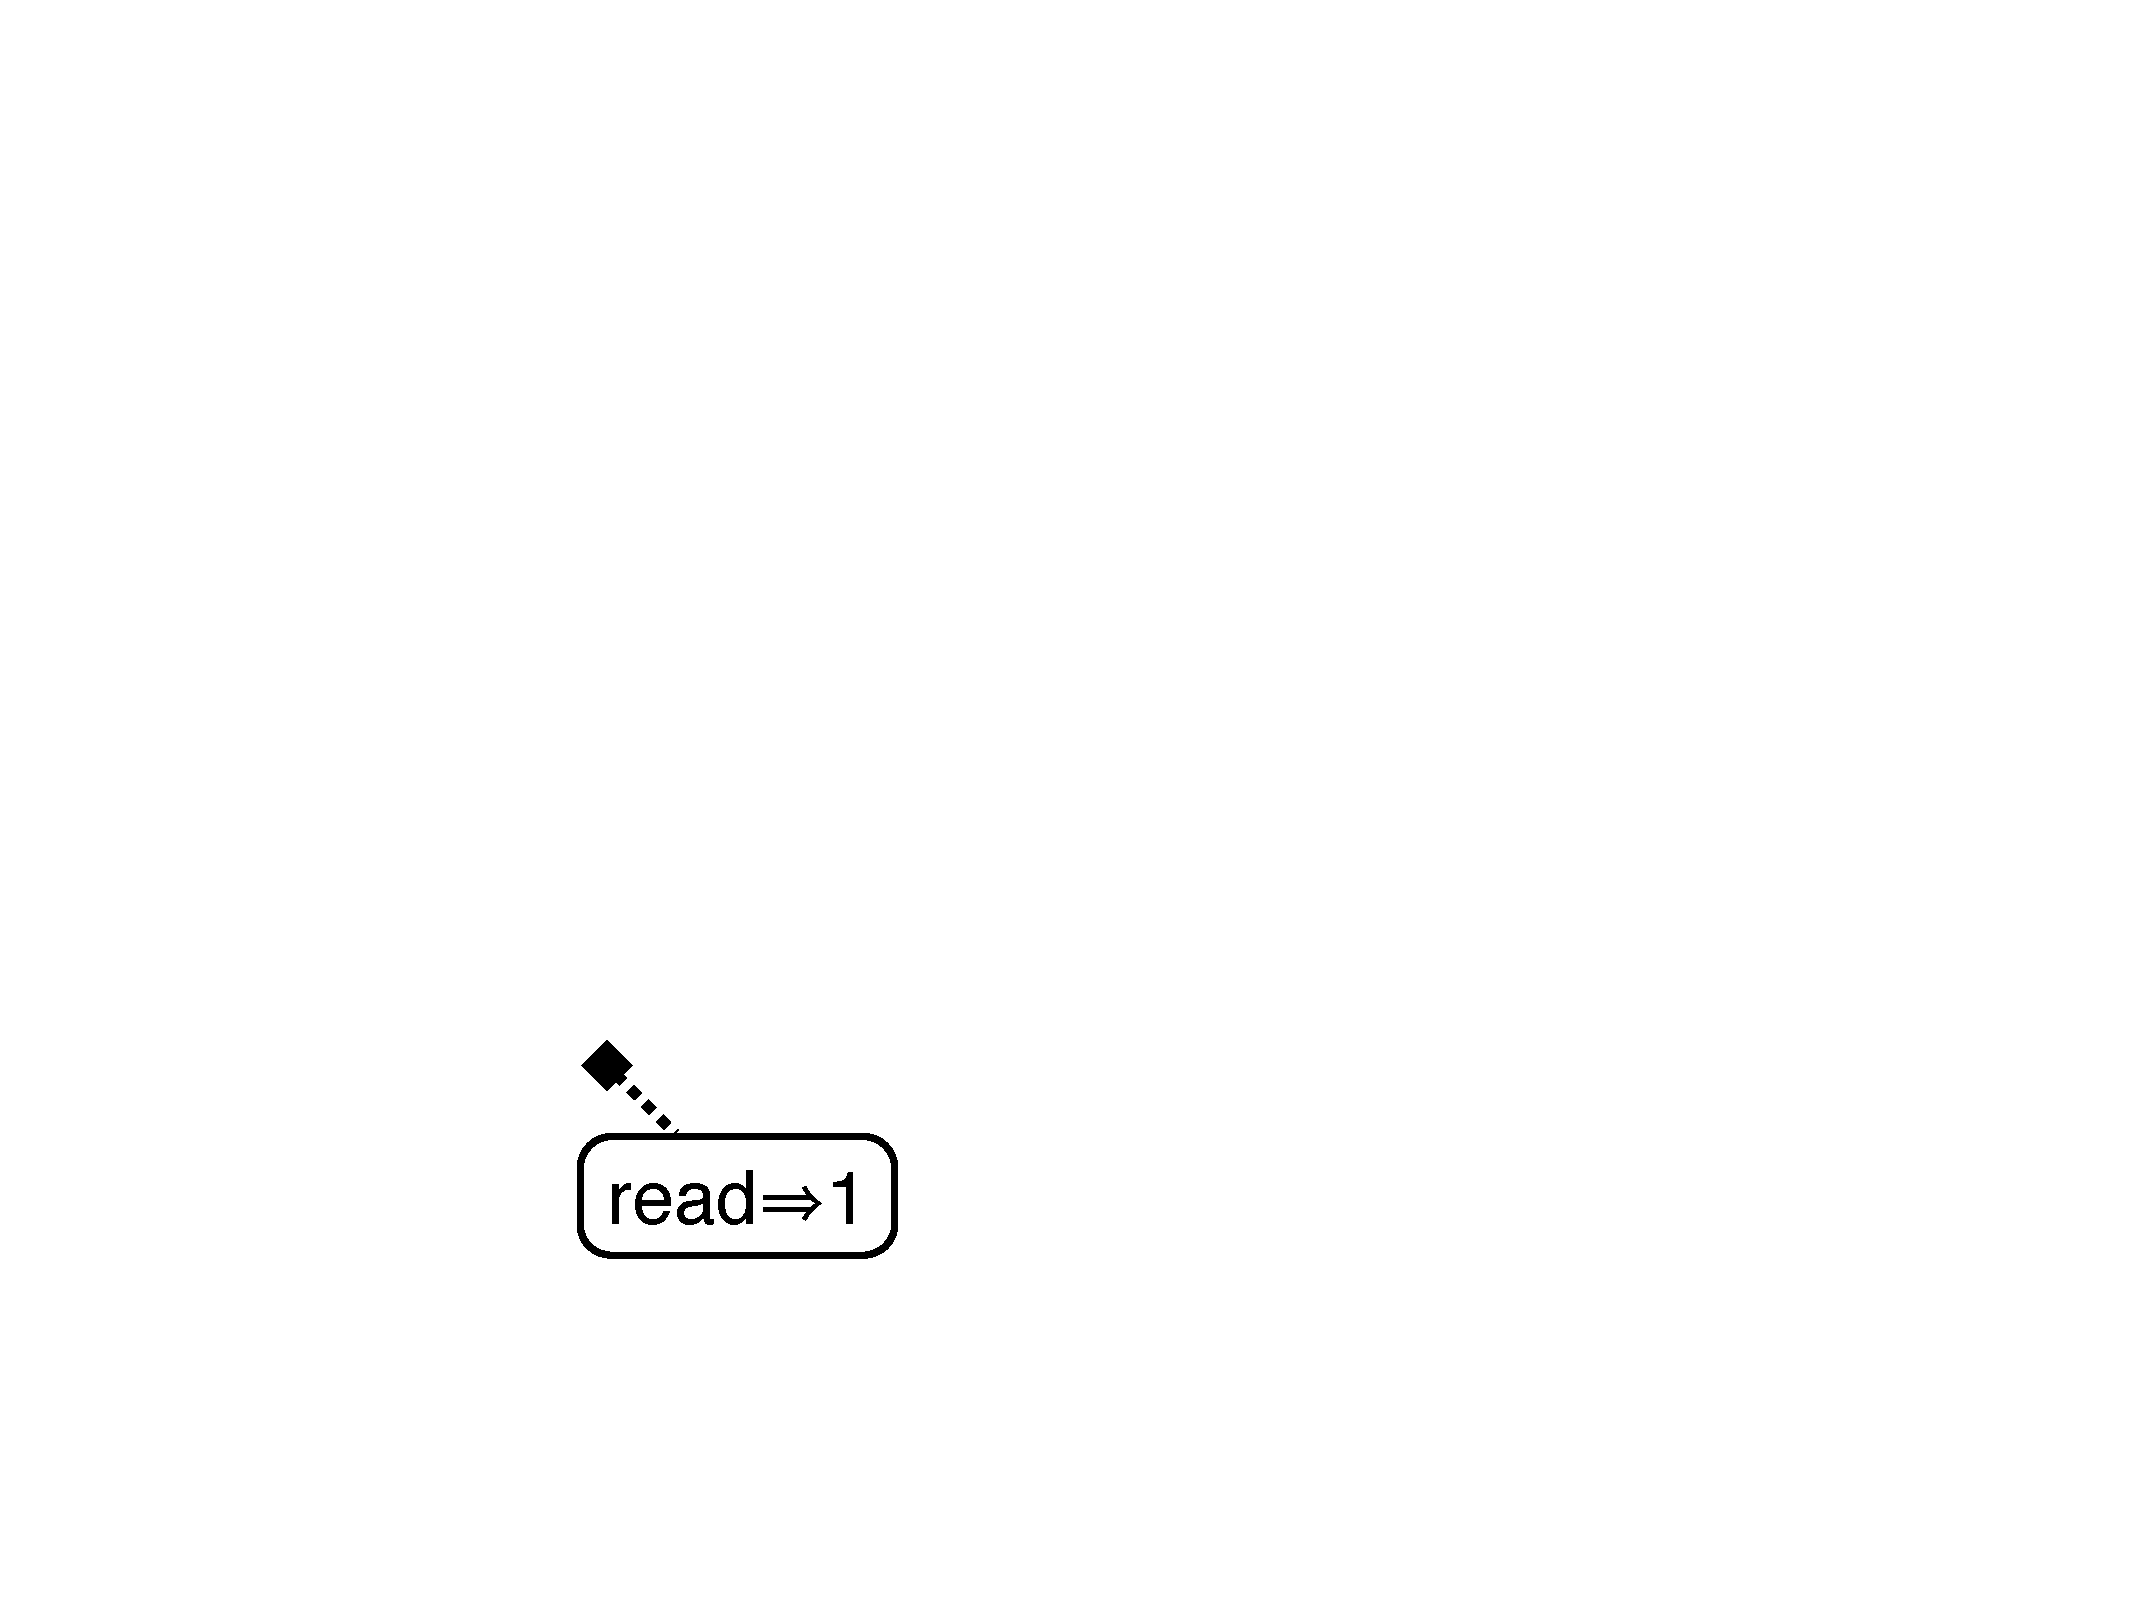
\includegraphics[scale=0.2]{figures/register-pattern-1},
    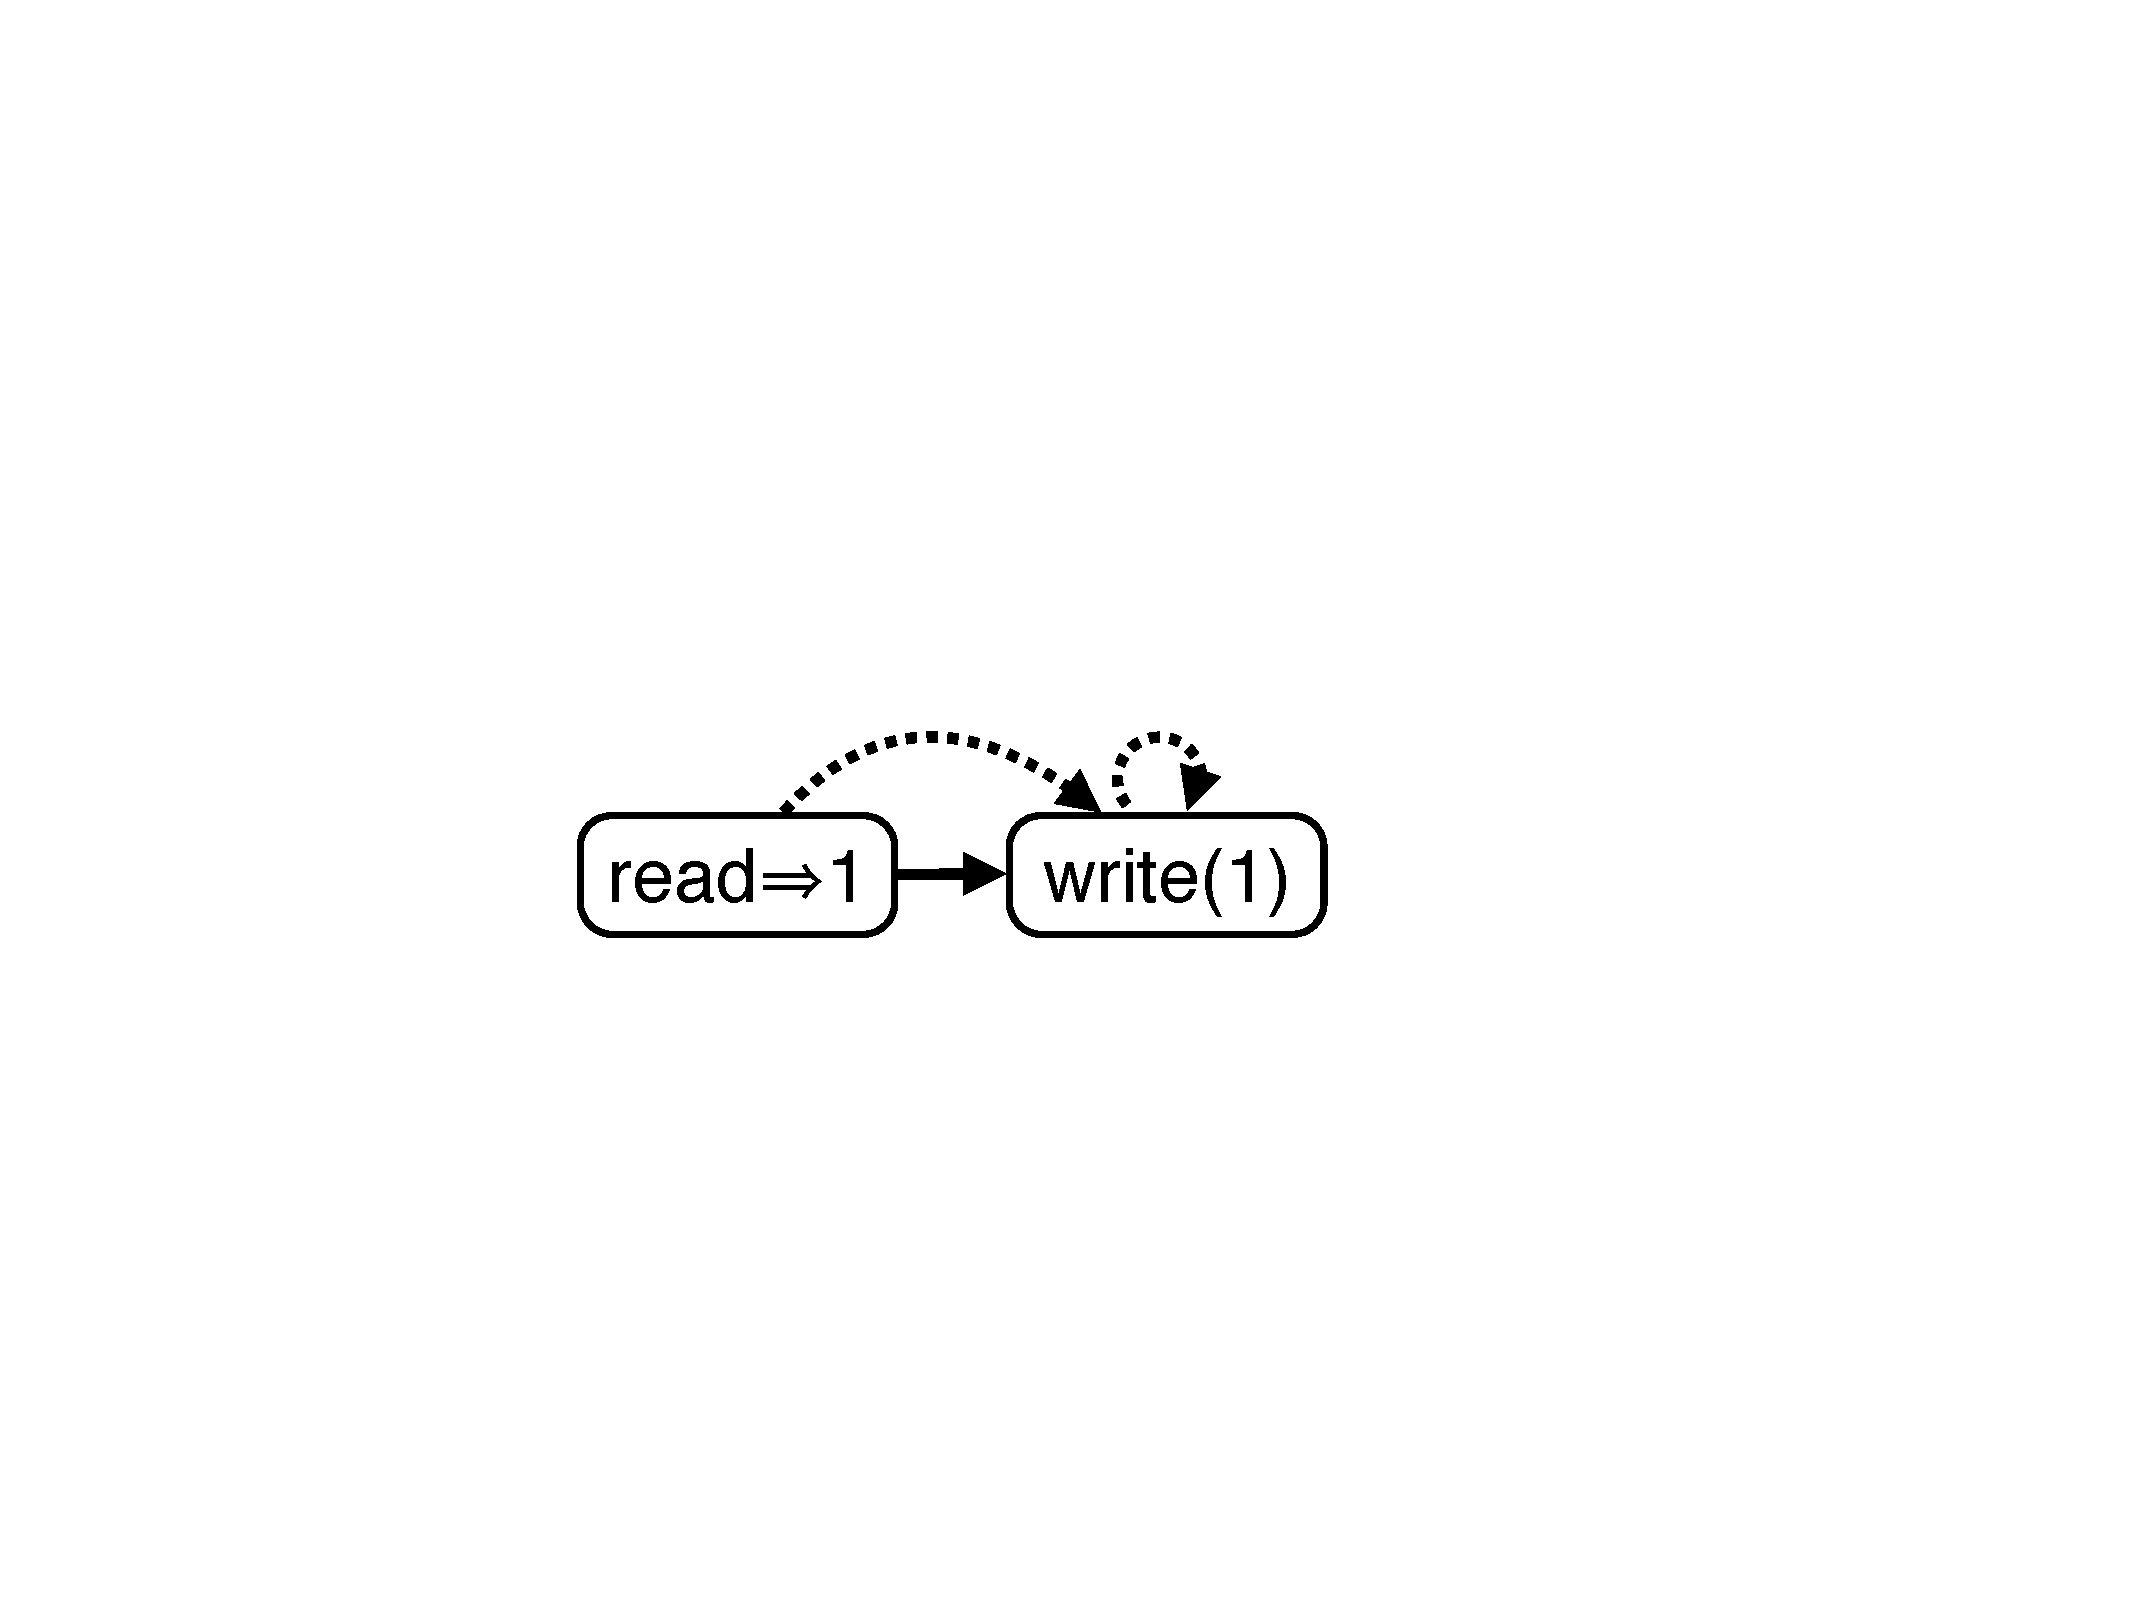
\includegraphics[scale=0.2]{figures/register-pattern-2},
    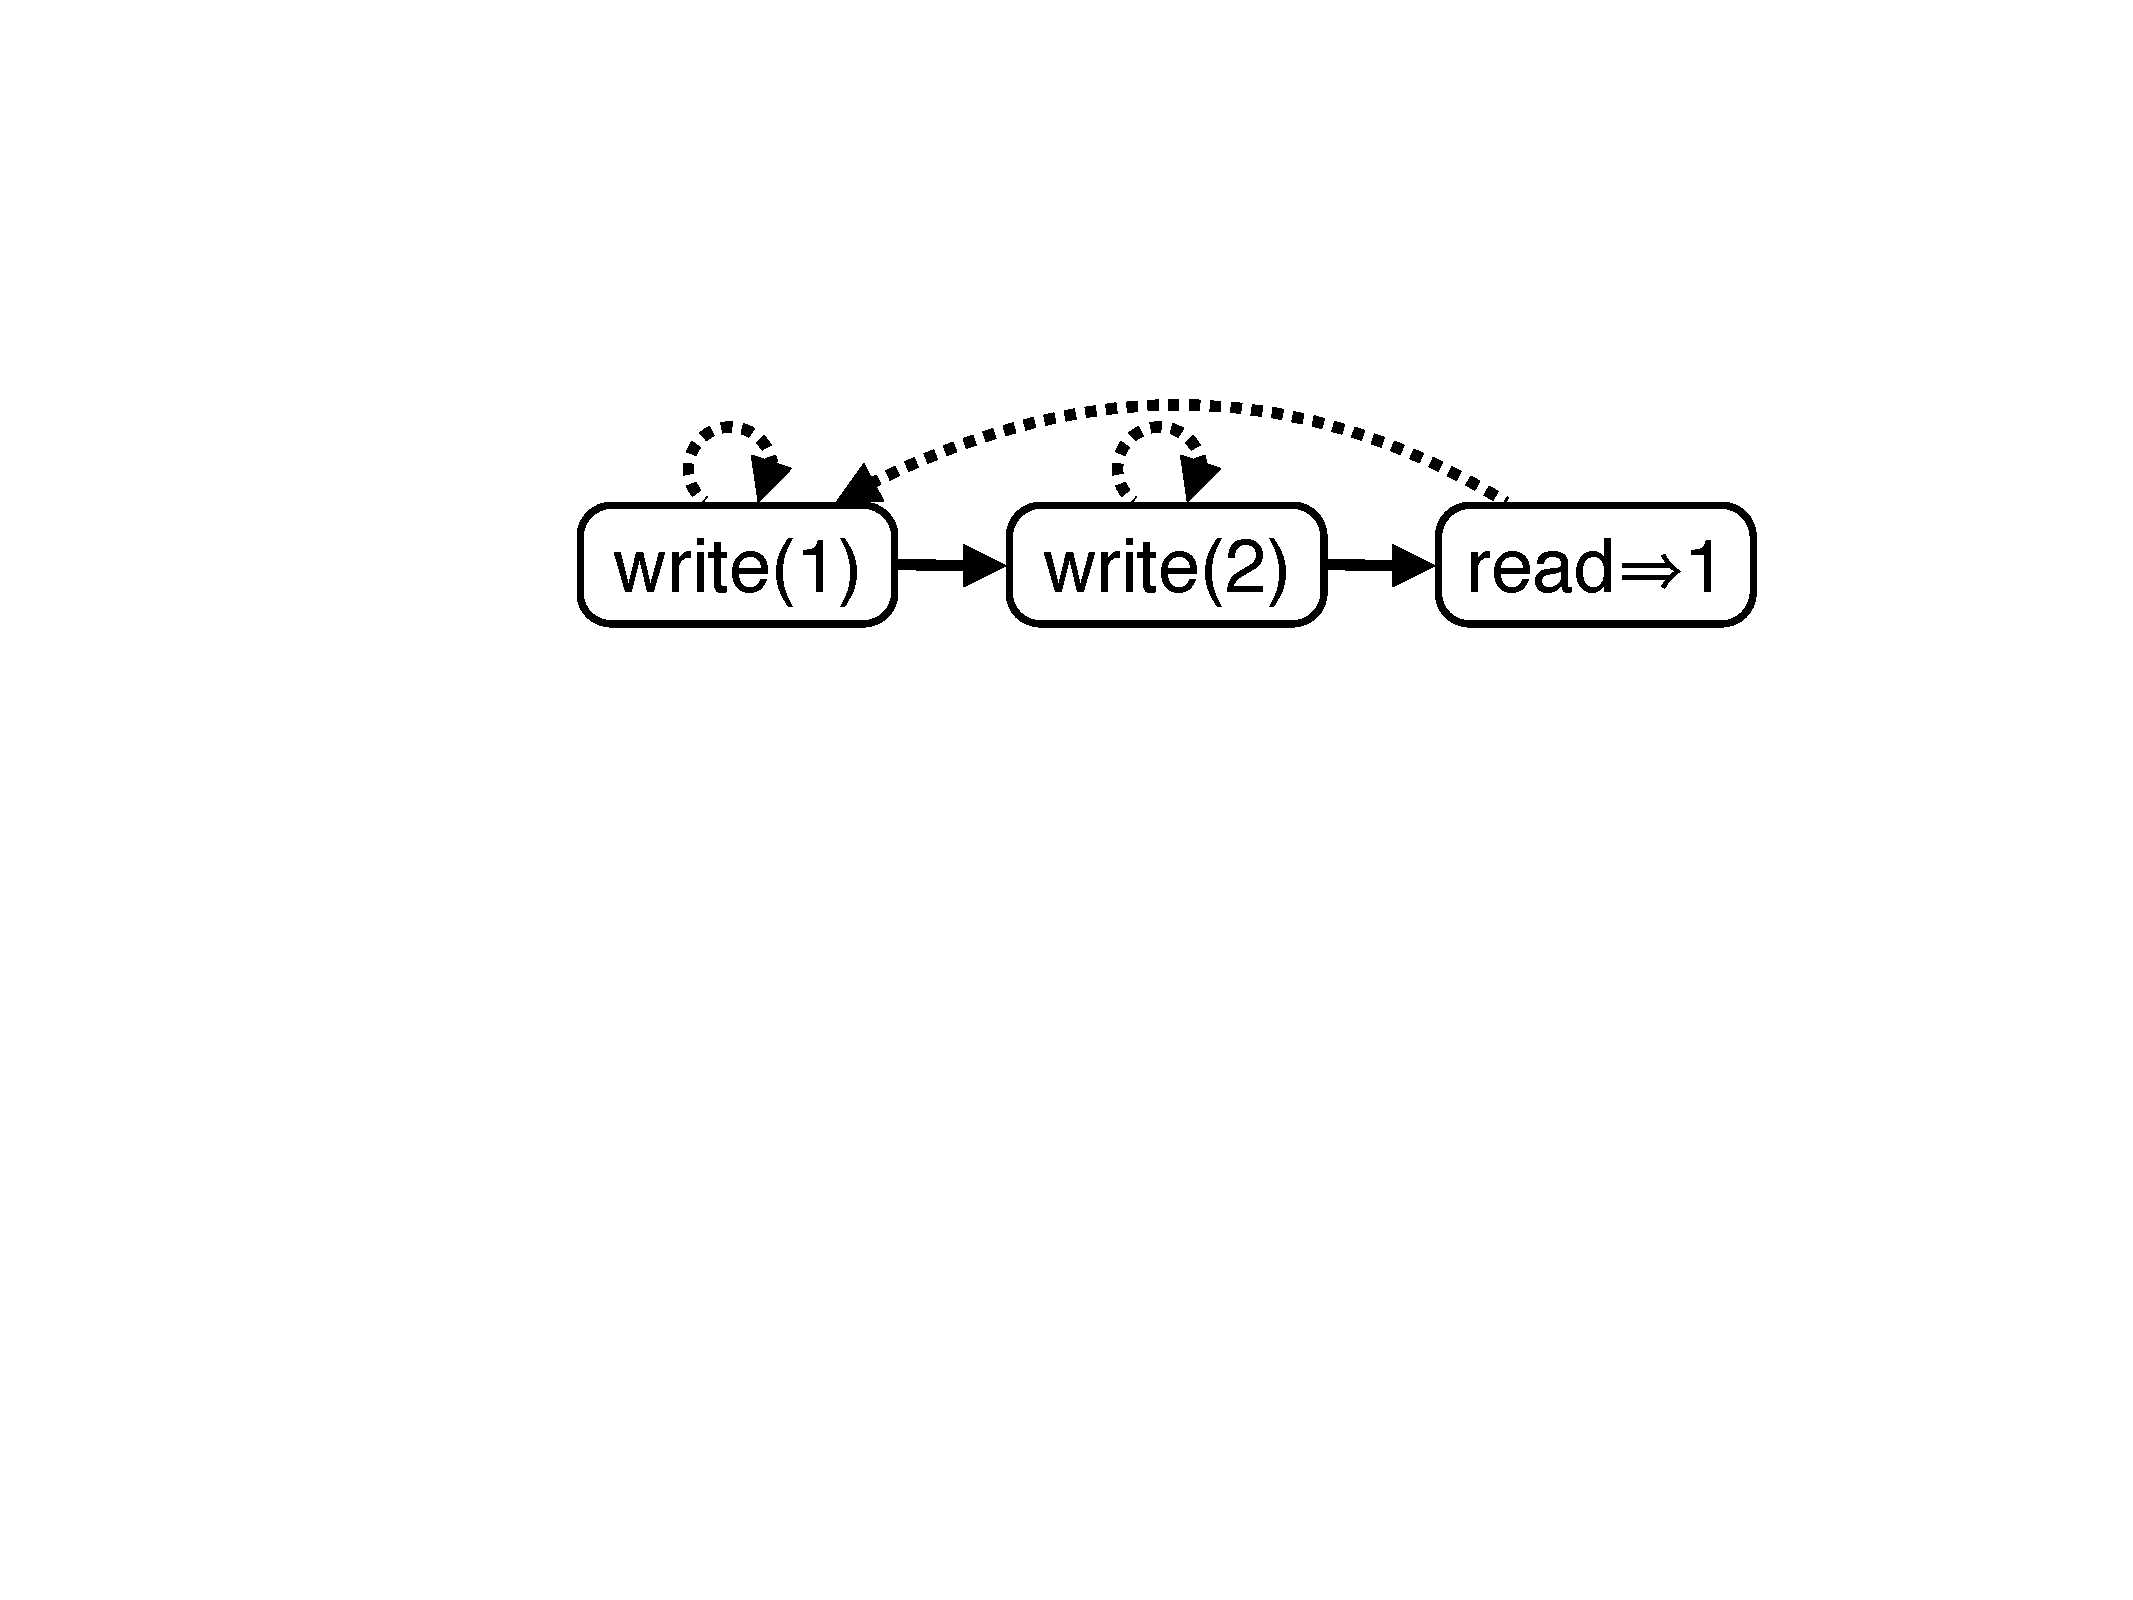
\includegraphics[scale=0.2]{figures/register-pattern-3}
    \caption{Three histories which generate the complement of the atomic
      register ADT kernel.}
    \label{fig:register-patterns}
  \end{figure}

\end{example}
